% Example file for 137th Convention paper
\documentclass{aes137}
\hyphenation{Post-Script}
\renewcommand{\deg}{\,^{\circ}}
 
% paper title, authors, affiliations
\authors{Regina E.\ Collecchia\aff{1}, Jonathan S.\ Abel\aff{1}, Sean A.\ Coffin\aff{1}, Eoin Callery\aff{1}, Yoo Hsiu Yeh\aff{1}, Kyle S.\ Spratt\aff{2}, Julius O.\ Smith, III\aff{1}}
\affiliation[1]{Center for Computer Research in Music and Acoustics, Department of Music, Stanford University, Stanford, CA 94305 USA}
\affiliation[2]{Applied Research Laboratories and Department of Mechanical Engineering, The University of Texas at Austin, Austin, TX, USA.}
\correspondence{Regina Collecchia}{colleccr@ccrma.stanford.edu}
\lastnames{Collechia, Abel, Coffin, Callery, Yeh, Spratt, Smith}
\title{}
\shorttitle{Alleyway Acoustics}

\correspondence{Regina Collecchia}{colleccr@ccrma.stanford.edu}

\lastnames{Collecchia, Abel, Coffin, Callery, Yeh, Spratt, Smith}

\title{On the Acoustics of Alleyways}


\begin{abstract}
Alleyways bounded by flat, reflective parallel walls and smooth
concrete floors produce impulse responses which are unexpectedly rich
in texture, featuring a long lasting modulated tone and a changing
timbre much like the sound of a didgeridoo. This work explores
alleyway acoustics with acoustic measurements and presents a
computational model based on the image method. Alleyway response
spectrograms show spectral zeros rising in frequency with time, and a
modulated tone lasting noticeably longer than the harmonic series
associated with the distance between the walls. With slight canting of
the walls and floors to produce the long lasting modulated tone, the
image method model captures much of this behavior.
\end{abstract}

\begin{document}

\maketitle % MANDATORY! 

\section{Introduction}

Narrow alleyways with flat, reflective, parallel walls and smooth,
reflective floors have remarkable acoustics, producing strong
harmonics and an evolving timbre. While the harmonics present are
similar to those of a small-diameter acoustic tube whose length is
equal to the wall spacing, the alleyway impulse response is much more
rich in texture, featuring a long lasting modulated tone and the
changing timbre of a didgeridoo. In this work, we study alleyway
acoustics through acoustic measurements and a computational model
based on the image method \cite{Borish} and the well established
theory of acoustic ducts \cite{Morse}.

% Finally, image method models tuned to each alleyway are presented, and their acoustic characteristics compared to the measurements.

\section{Measurements}

Acoustic measurements were made in three alleyways in Palo Alto, CA
with balloon pops, hand claps, and a small clapper similar to an
orchestral whip as sound sources, recorded with INSERT RECORDING EQUIP
HERE (iphone, handheld recorder, interface, capsule mics). One was
measured with slow logarithmic sine sweeps, recorded using a MOTU
Traveler Mk3 audio interface, K\&H speaker, and two C-414
microphones. The locations of the microphones and speaker for the sine
sweep impulse response collection in an alleyway adjacent to Printer's
Ink Cafe is shown in Fig.~1.

\begin{figure} 
\begin{minipage}[b]{0.46\linewidth} \centering
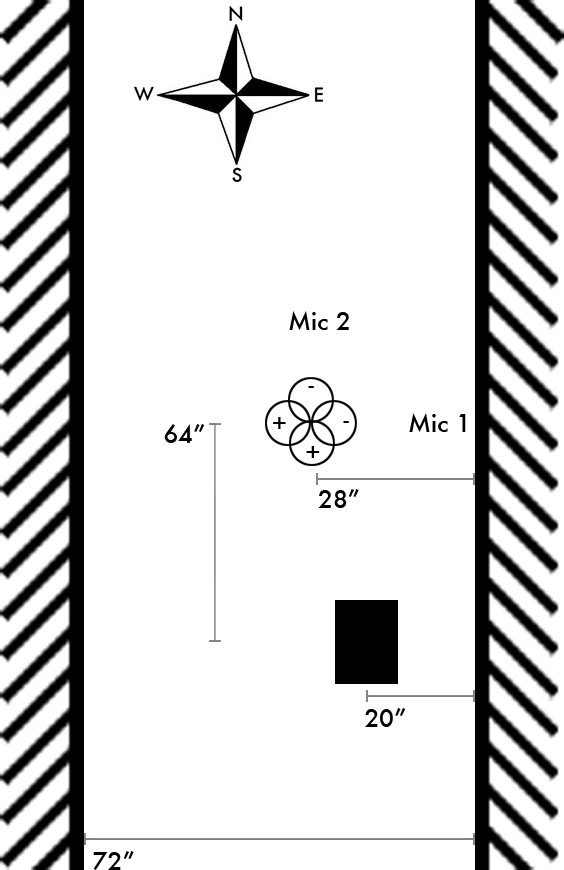
\includegraphics[width=\textwidth]{images/alleyway_birdseye.png}
\end{minipage}
\hspace{0.1\linewidth}
\begin{minipage}[b]{0.41\linewidth} \centering
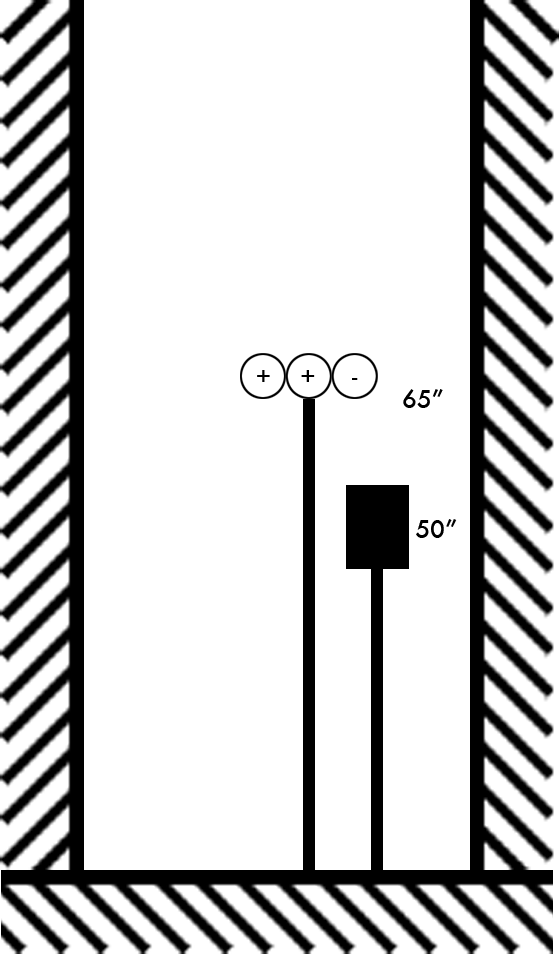
\includegraphics[width=\textwidth]{images/alleyway_lookingdown.png}
\end{minipage}

\caption{Plan view (left) of our setup in ``Printer's Ink Alleyway"
  with a K\&H speaker and pair of figure-8 C-414 microphones; and
  elevation view of the alley (right). Measurements were made with
  speaker oriented to the North, East, and West in this position.}
\end{figure}

Measurements were made using a number of source and microphone
positions, including positions between and at the walls and at various
heights ranging from on the ground to eye level. All measurement
frequency responses show peaks at the harmonic series associated with
the distance between the parallel walls, given explicitly in the table
and FFT plots below (Figs.~2-4).

\begin{center} \begin{table}[h!]
\footnotesize
\begin{tabular}{|l|c|c|c|}
\hline
\textbf{Adjacent Store} & \textbf{WxLxH} & \textbf{Wall cant} & \textbf{Floor dip} \\
\hline
Printer's Ink & 1.85 x 19.69 x 7.38m & Yes (left): $\approx0.52\deg$ & 0m \\
\hline
Accent Art & 2.46 x 24.62 x 6.77m & $0.2\deg$ & 0m \\
\hline
Mac's Smoke Shop & 2.46 x 24.62 x 7.38m & Yes (right): $\approx0.30\deg$ & 0.077m \\
\hline
\end{tabular} \caption{Dimensions of the three measured alleyways, named for the business adjacent to them.} \end{table}
\normalsize
\end{center}

% FFT plots

\begin{figure}[h!] \centering 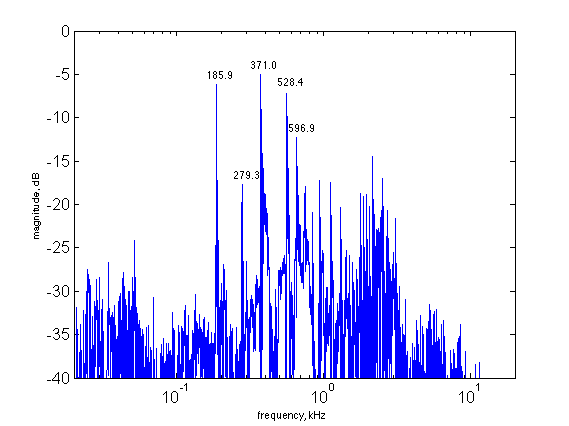
\includegraphics[width=\linewidth]{images/printers_labeled_IR.png} \caption{Resonant frequencies of the Printer's Ink Alley from a balloon pop recorded with INSERT HANDHELD RECORDER. The labeled peaks have a difference of either 90 or 180Hz, related to its width (1.85m $\simeq$ 185Hz).} \end{figure}

\begin{figure}[h!] \centering 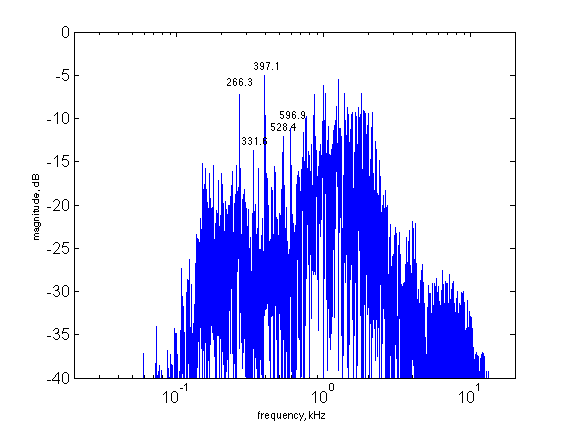
\includegraphics[width=\linewidth]{images/artists_labeled_IR.png} \caption{Resonant frequencies of the Artist Accent Alley from hand claps recorded with an iPhone 5S. These differ in either 66 or 132Hz, related to its width (2.46m $\simeq$ 139Hz).} \end{figure}

\begin{figure}[h!] \centering 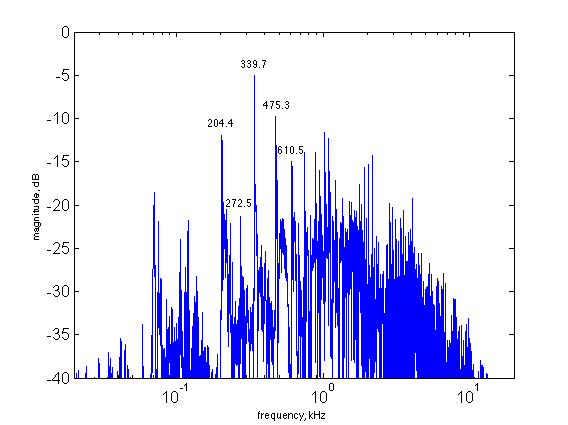
\includegraphics[width=\linewidth]{images/macs_labeled_IR.png} \caption{Resonant frequencies of the Mac's Smoke Shop Alley from a balloon pop recorded with INSERT RECORDING DEVICE, differing in either 68 or 135Hz, again related to its width (2.46m).} \end{figure}

The impact of the vertical resonant frequencies is better seen in the spectrograms of these impulse responses. % , as they should be around 10Hz for the 8m tall walls...

\section{Modal analysis}
Modal analysis connects the resonant frequencies seen in the different alleyways with their physical dimensions. Duct modes, etc.

\section{Transient response}
All measurement spectrograms (Figs.~5 and 6) showed weak spectral
zeros between the ``wall" harmonics ($\approx$185 Hz and multiples for
a 1.85m-wide alleyway) that rise in frequency with time, and a
modulated tone ($\approx$370 Hz for the 1.85m-wide alleyway) lasting
noticeably longer than the harmonic series associated with the
distance between the walls.

\begin{figure}[h] \centering 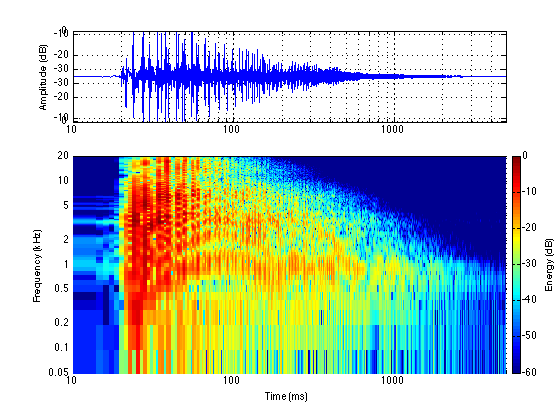
\includegraphics[width=\linewidth, trim=10mm 5mm 2mm 7mm, clip]{images/logspectrogram.png} \caption{Logarithmic time scale spectrogram for a measured impulse response, speaker oriented to the West, microphone channel 1.} \end{figure}

At the onset of the energy, the response rises and then falls back
down within the first 100 milliseconds. The tone modulation rate was
roughly 1.2 Hz, indicating the presence of two modes, very close in
frequency. The harmonic series lasted a few hundred milliseconds,
whereas the tone lasted several seconds. Fig.~6, with a linear time
scale, shows more detail of these modulating modes.

\begin{figure}[h!] \centering 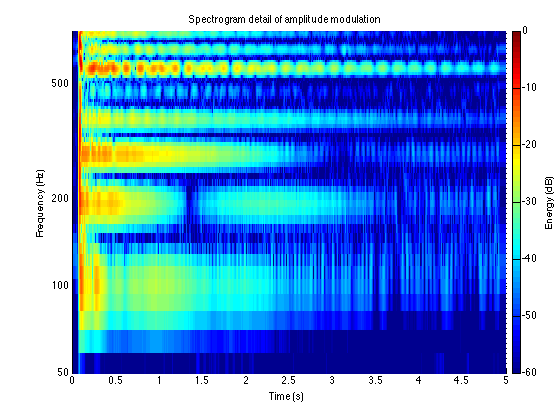
\includegraphics[width=\linewidth, trim=10mm 5mm 2mm 3mm, clip]{images/logspectrogram_evenmoredetail.png} \caption{Spectrogram with linear time scale of a balloon pop of the same impulse response as Fig.~2, showing more detail of the low frequencies and their strong, independent modulation.} \end{figure}

Energy decay envelope, etc.

\section{Image model}

The simple geometry of an alleyway with all surfaces meeting at right
angles places image sources in rows parallel to the ground and
perpendicular to the walls, with pairs of image sources spaced every
two alleyway widths apart. At high frequencies, the open alleyway top
is not reflective, and there are two rows, one at the height of the
source, and another below the ground at a depth equal to the negative
source height (Fig.~7). At low frequencies, the top of the alleyway
presents an inverting reflection, and there will be a series of image
source rows above and below the ground, spaced about even multiples of
the alleyway height.

\begin{figure}[h!] \centering 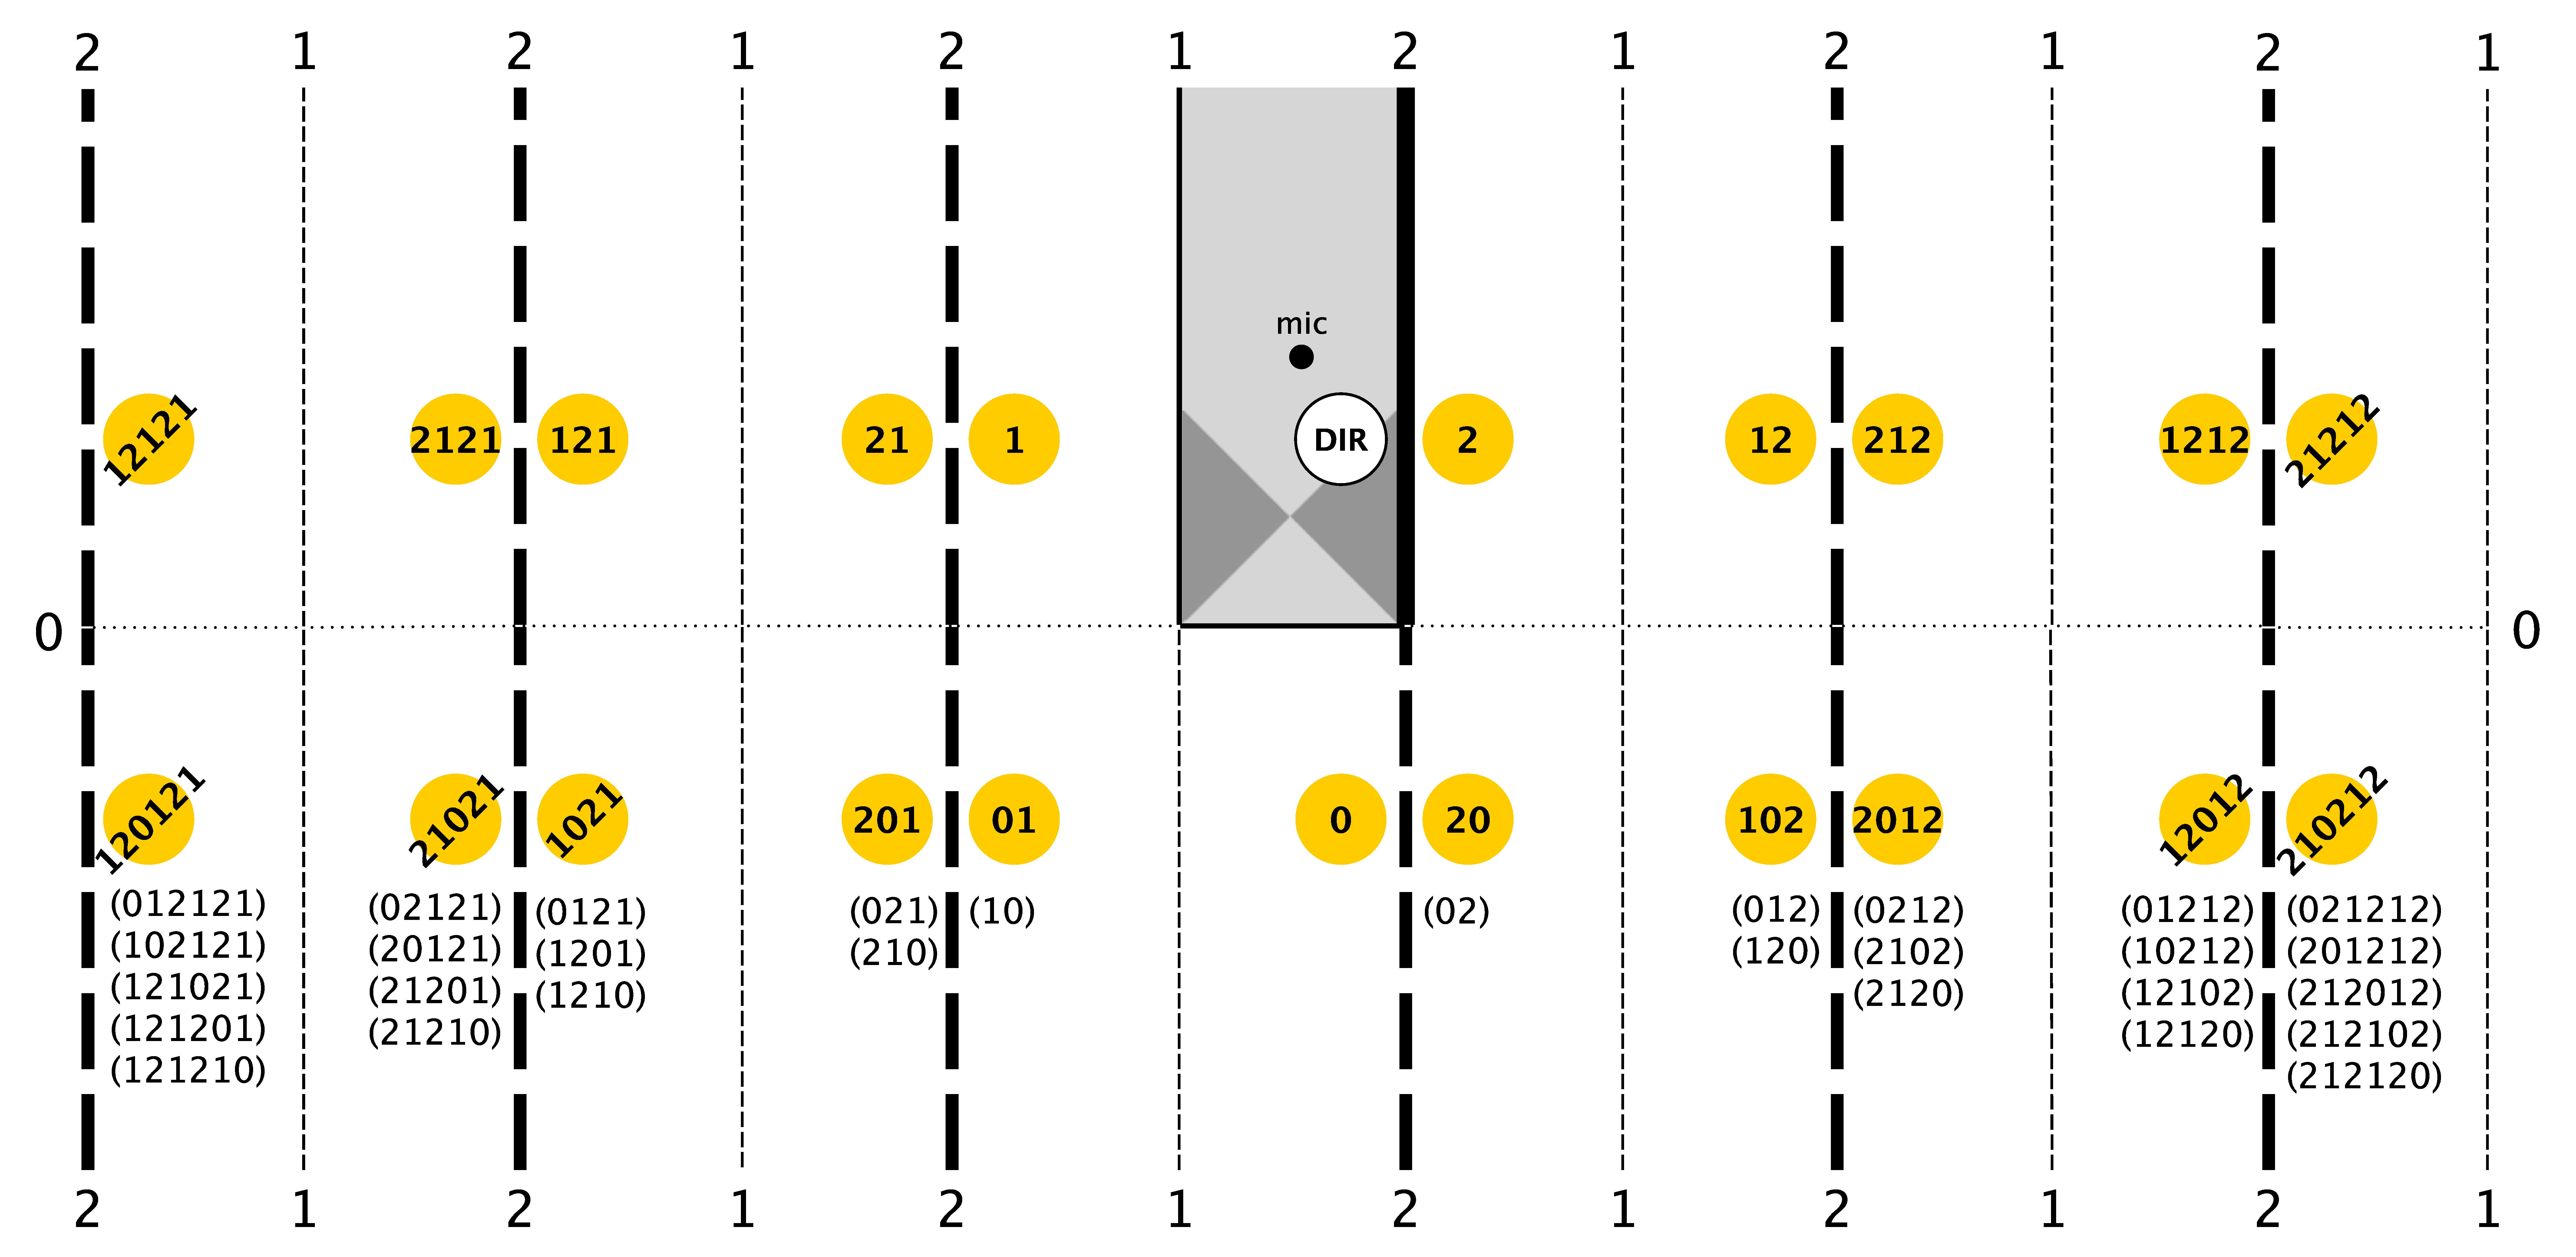
\includegraphics[width=\linewidth]{images/ISM_uncanted.pdf} \caption{The image source model for an alley with perfectly orthogonal walls.} \end{figure}

This simple model describes pretty closely what we see in the first 75
milliseconds of the impulse response, proven by annotating a measured
impulse response with the expected arrival of reflections from the
virtual sources in Fig.~8. Measurements taken with figure 8
microphones orthogonal to one another show arrivals from the West wall
as positive spikes and arrivals from the East as negative ones. The
very first early reflections hit the microphones near their pole, as
well as the direct path, so these events are more evident in the
second channel, pointed down the length of the alley. Considering the
microphone antennae pattern, speaker radiation pattern (facing the
West wall), and speed of sound in air, we can relate visible peaks in
the impulse response to virtual sources in our model.

\begin{figure}[h!] \centering 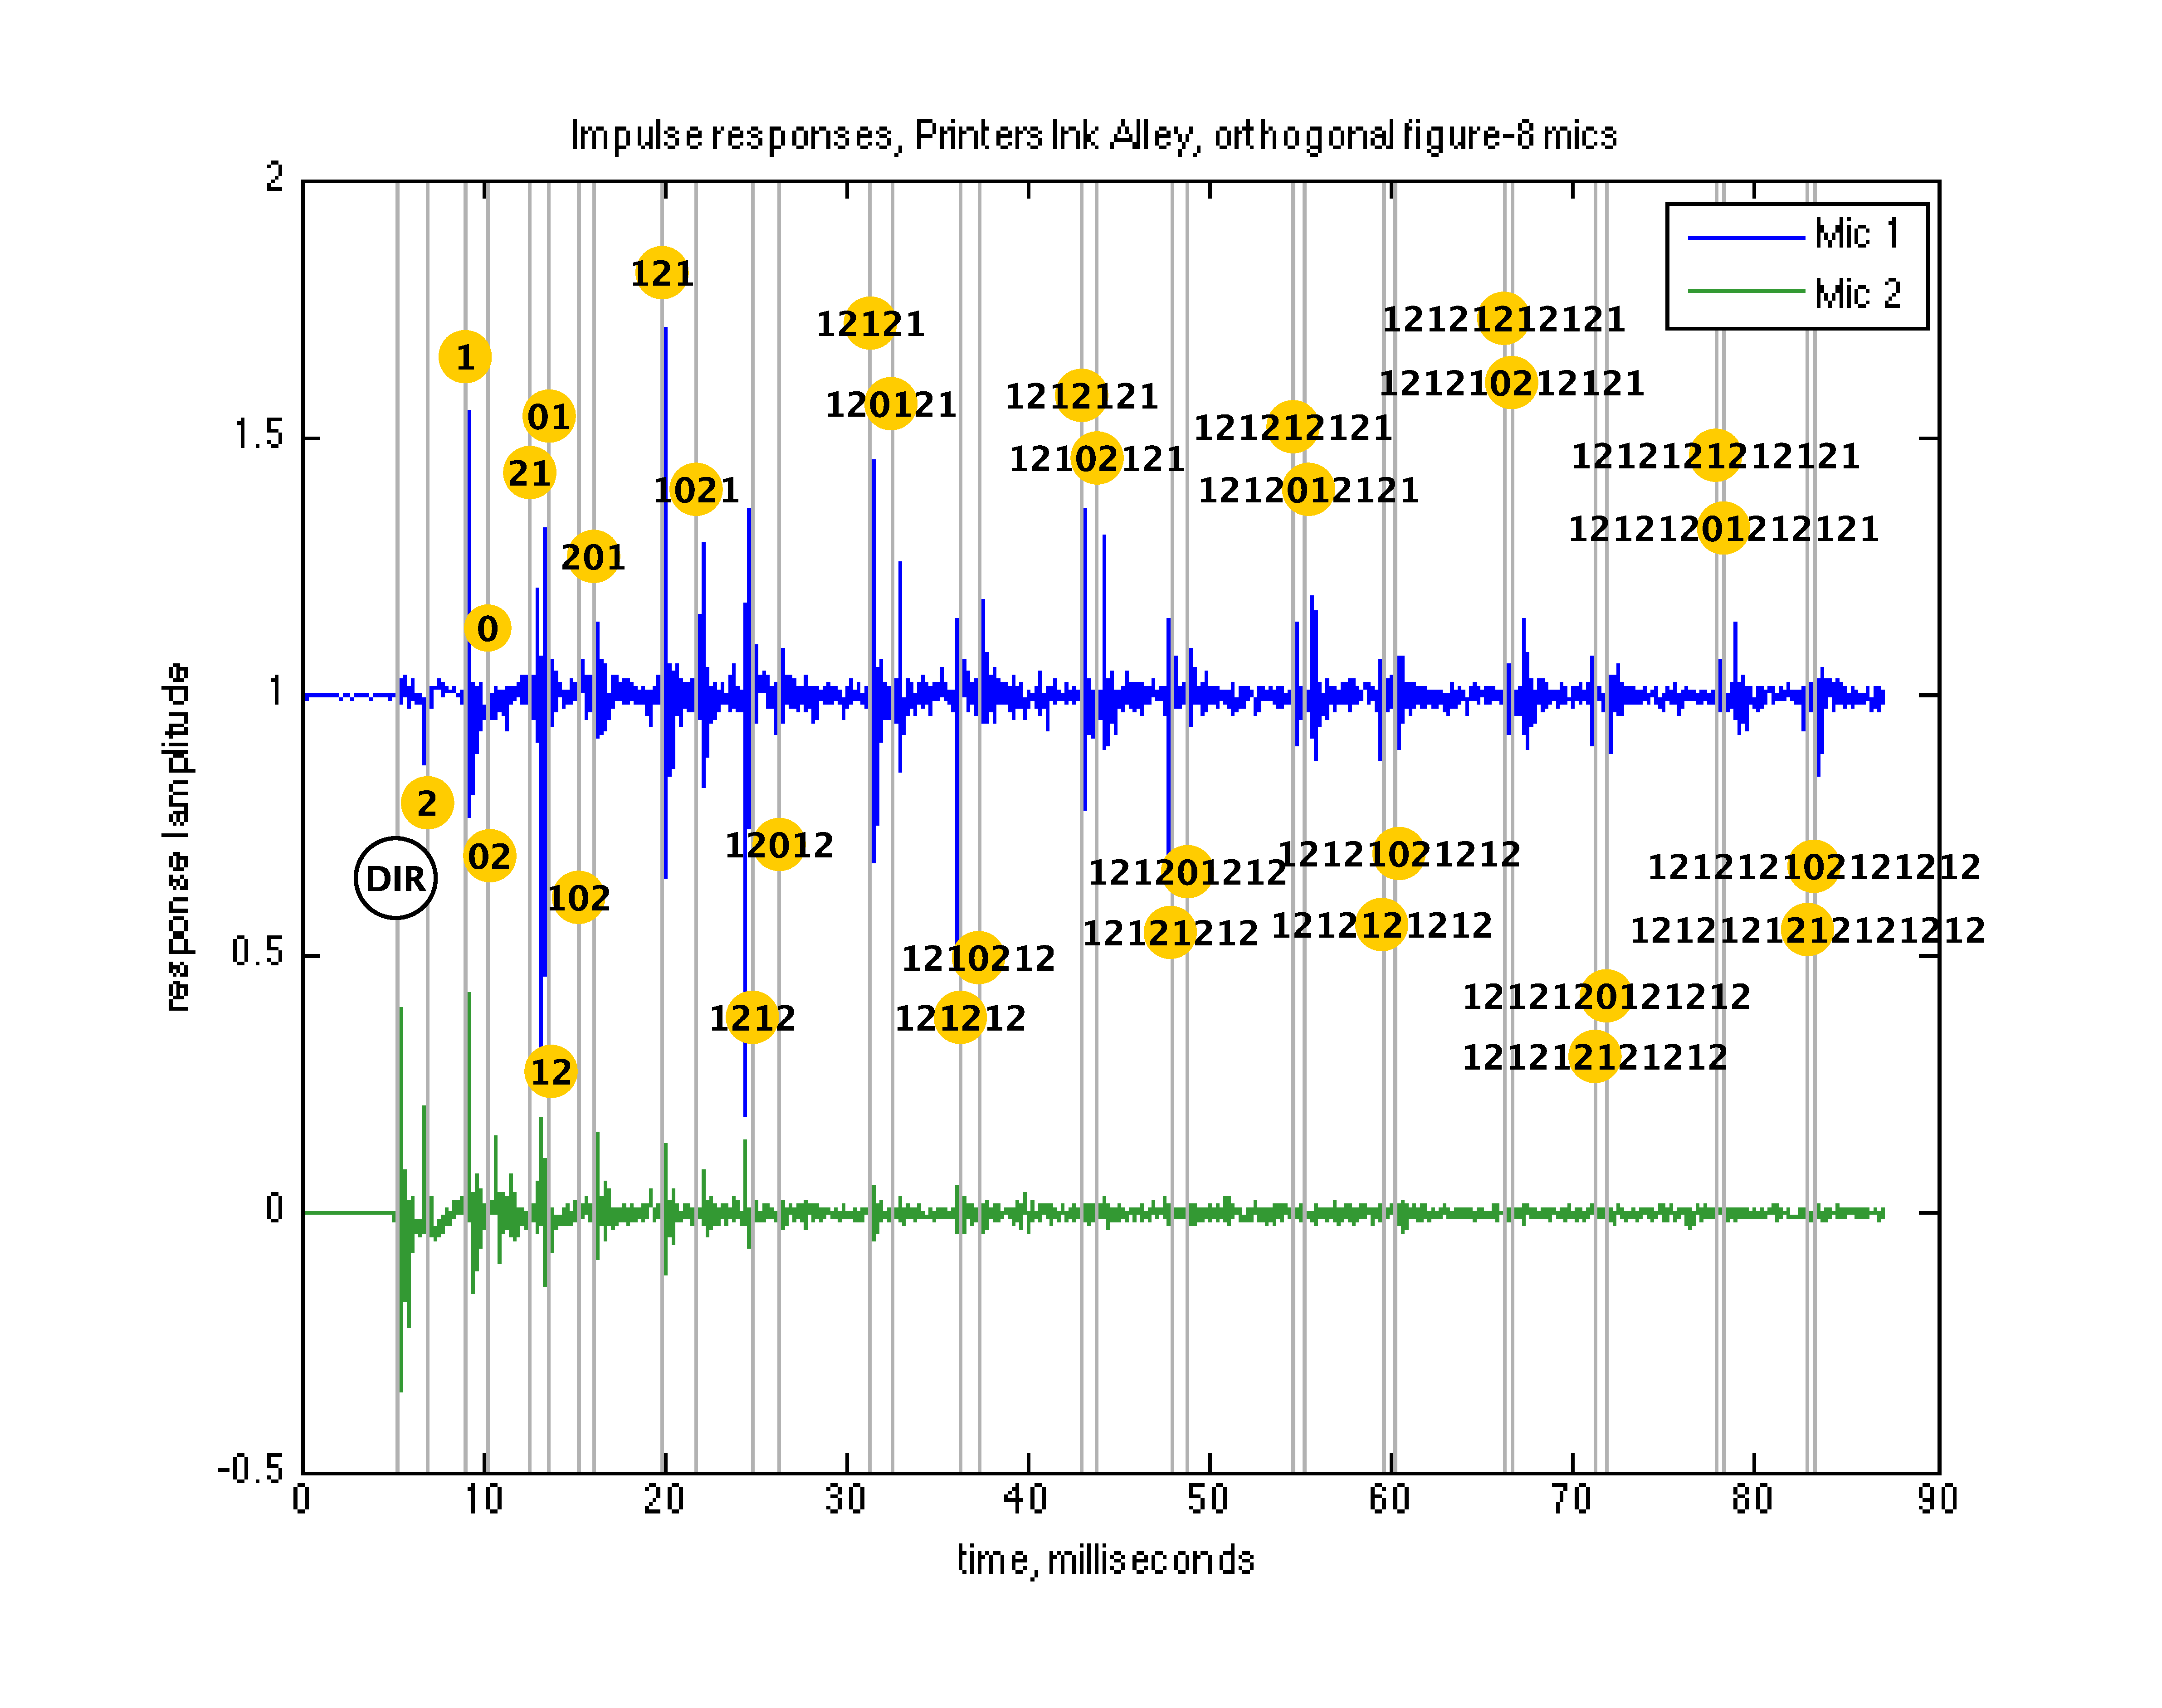
\includegraphics[width=\linewidth]{images/annotated_reflections_v2.pdf} \caption{Impulse response for the setup shown in Fig.~1 with speaker oriented to the West, annotated with the virtual sources from our model. Gray vertical lines mark the expected time of arrival of reflections coming from virtual sources, and the yellow circles label the virtual source index. After about 20ms, the sources originating from behind the speaker (e.g., reflecting off of Wall 2) are less evident. The direct path, first reflection off of Wall 2, and earliest reflections off of the floor are also small in Mic 1, as these arrived in the null of the figure-8 pattern which was oriented towards the parallel walls.} \end{figure}

%\begin{figure} 
%\begin{minipage}[b]{0.45\linewidth} \centering
%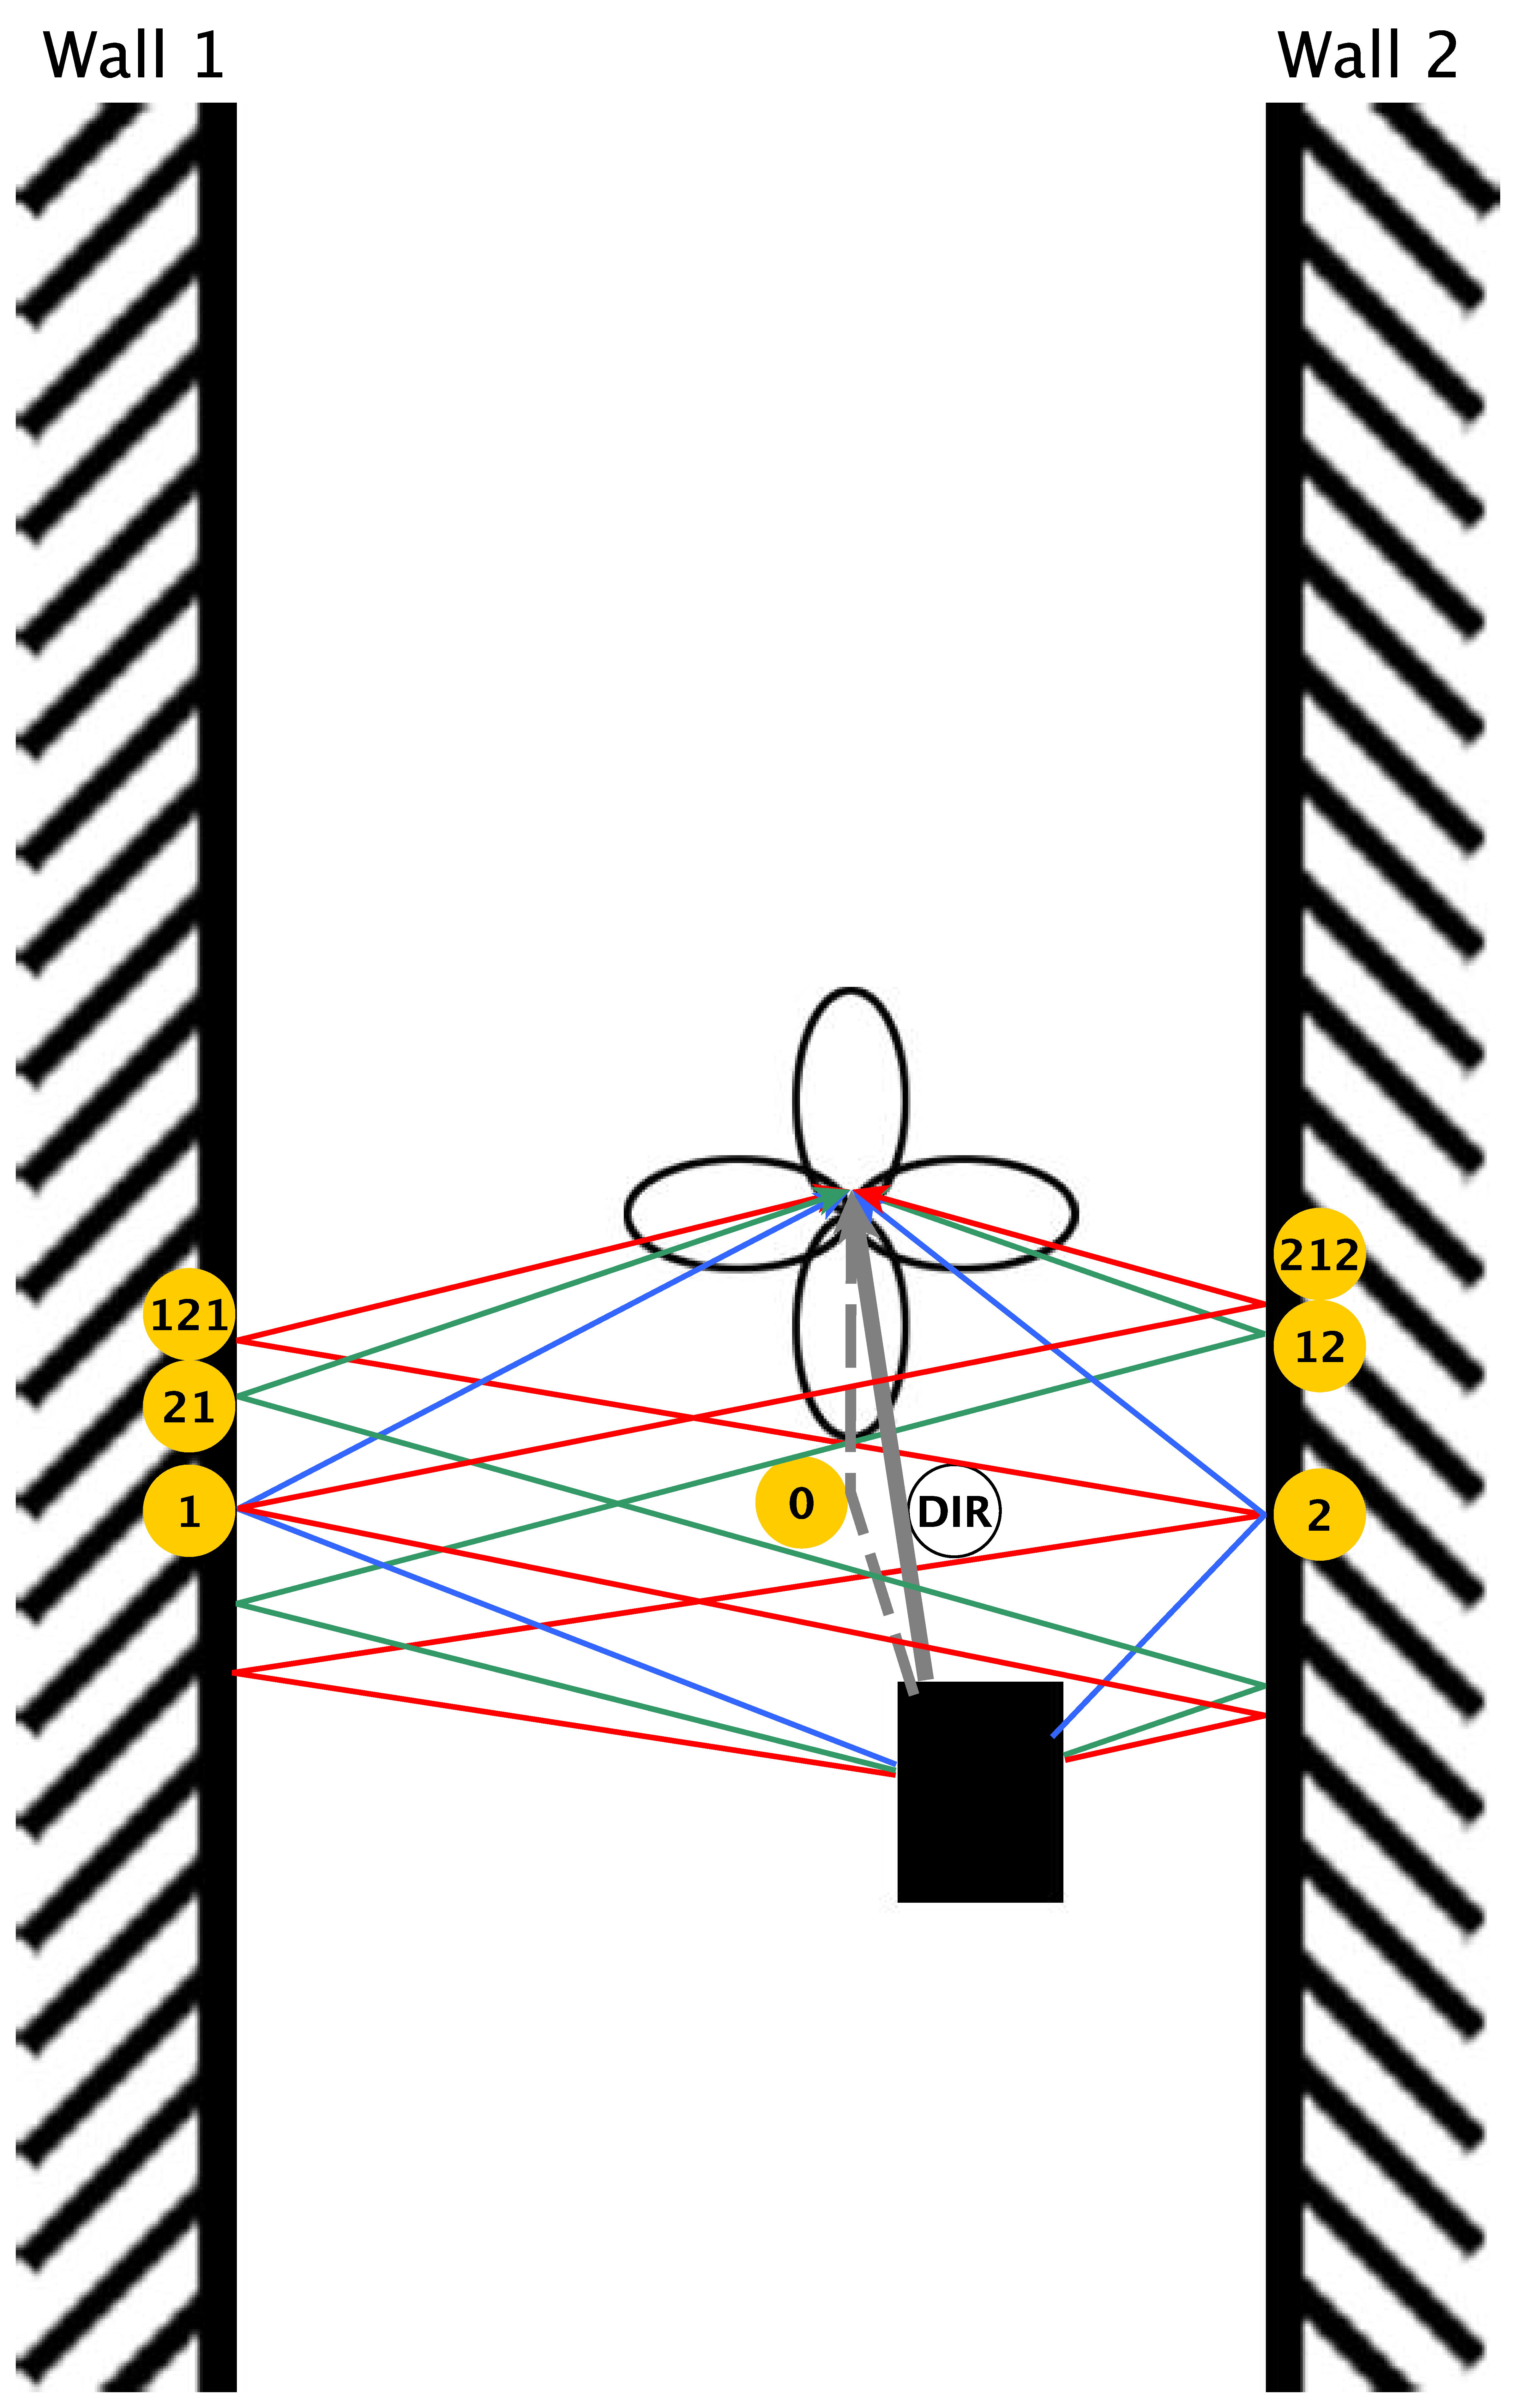
\includegraphics[width=\textwidth]{images/planview_paths.pdf}
%\end{minipage}
%\hspace{0.1\linewidth}
%\begin{minipage}[b]{0.43\linewidth} \centering
%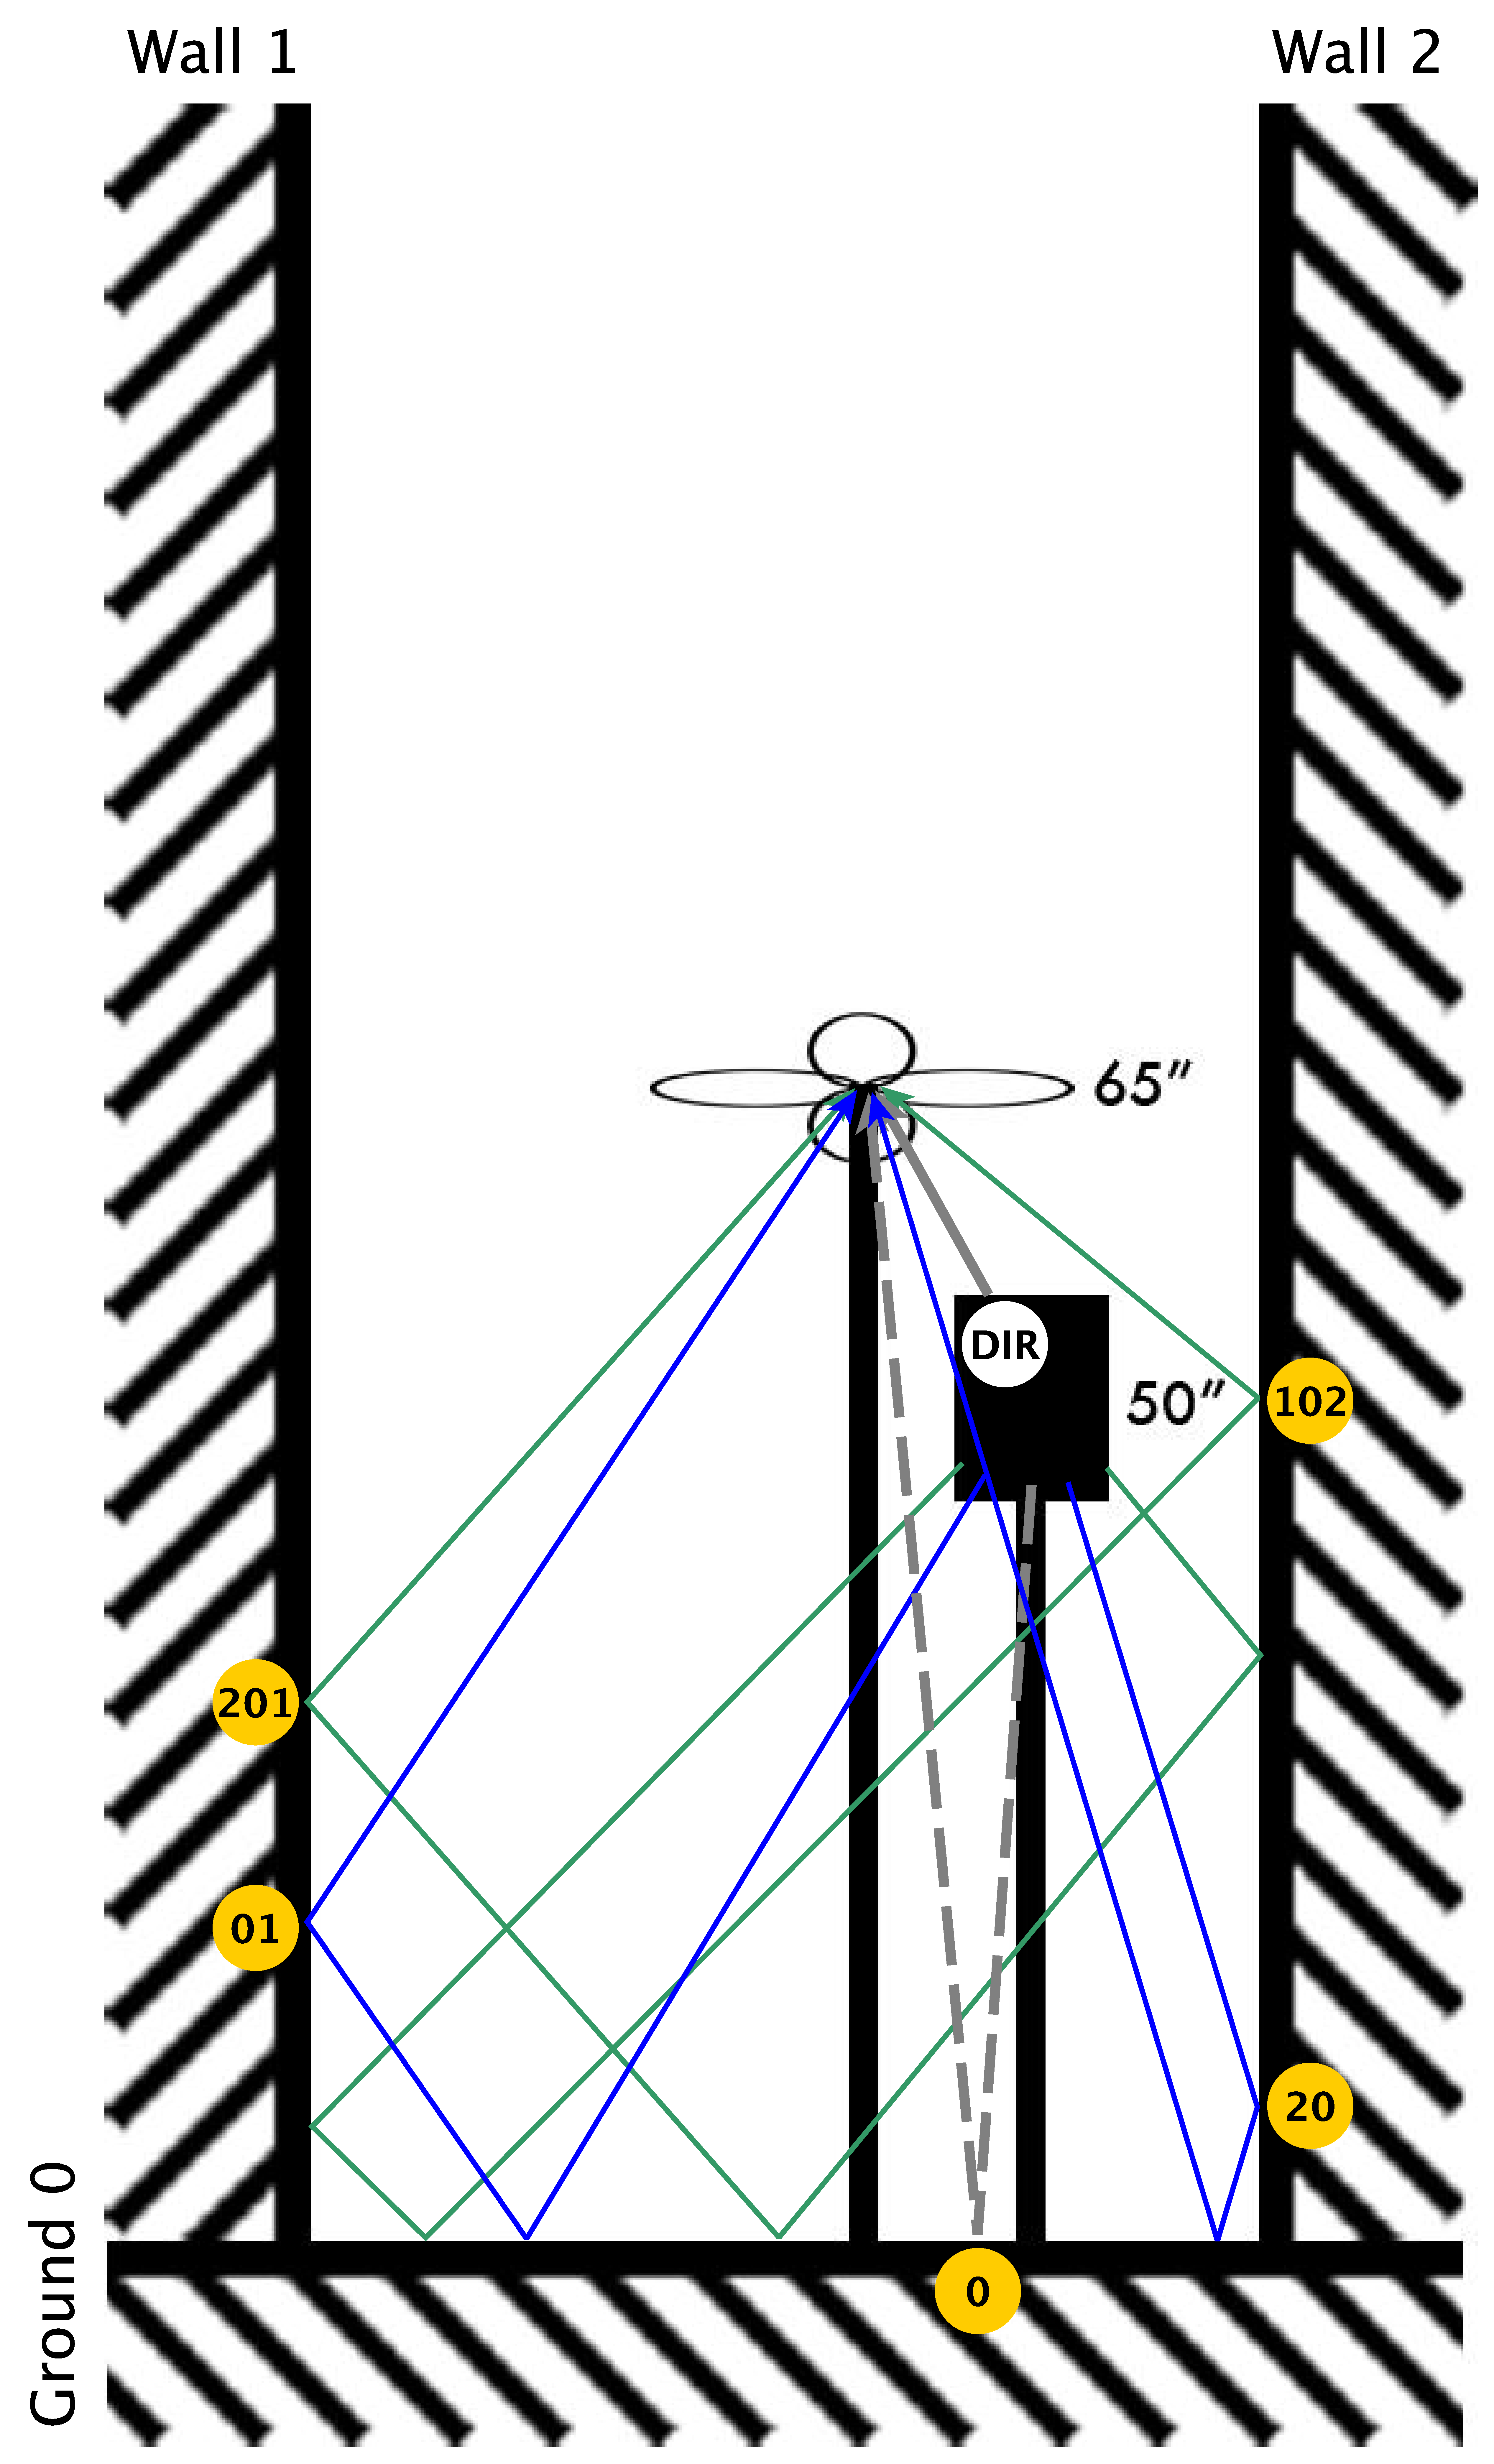
\includegraphics[width=\textwidth]{images/elevationview_paths.pdf}
%\end{minipage}
%\caption{Plan view (left) of our setup in ``Printer's Ink Alleyway" with speaker and pair of figure-8 microphones, and elevation view of the alley (right). Measurements were made with speaker oriented to the North, East, and West.}
%\end{figure}

\begin{figure}[h!] \centering 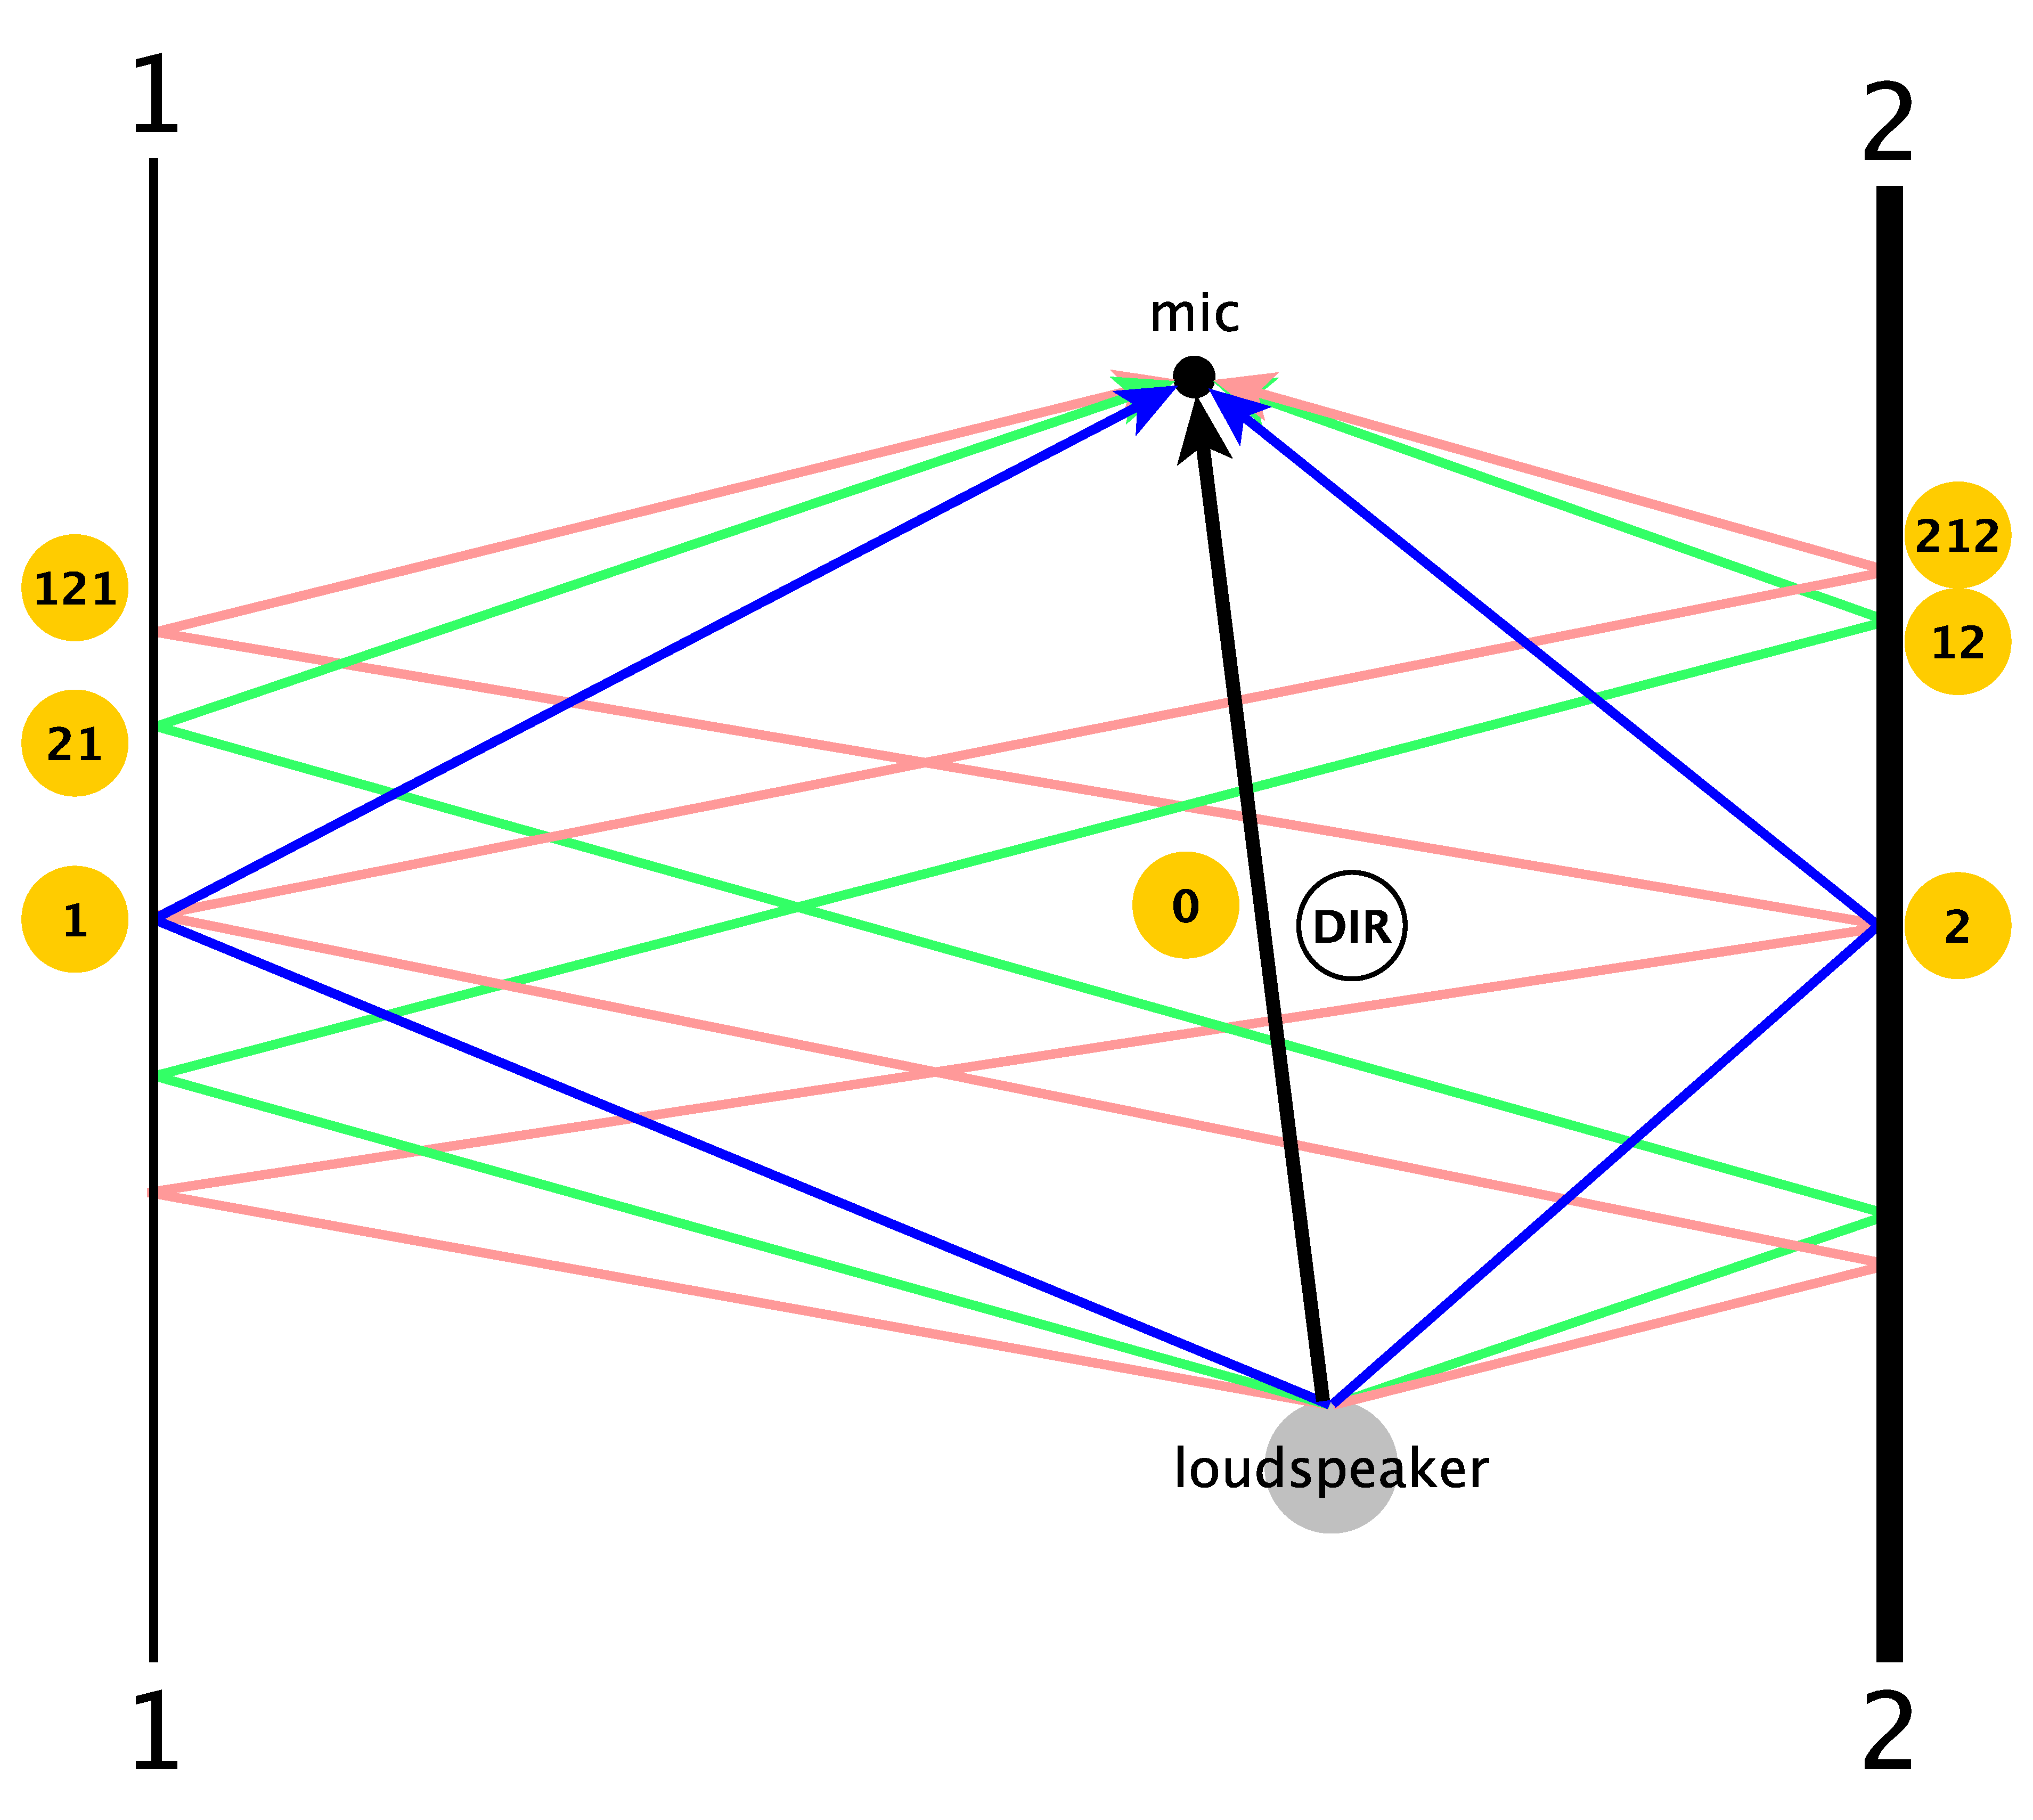
\includegraphics[width=0.7\linewidth]{images/planview_paths_v2.pdf} \caption{The first three orders of reflections as viewed from above the alley.} \end{figure}


As you can see, after the `201' source, no more sources beginning with
`2' (implying that they originated from the back of the speaker) are
labeled, as they get lost in the noise. After the first handful of
reflections, a clear pattern emerges between the polarity of pulses
and the source location: sources with virtual location (x,y) and
(x,-y) come in pairs in the impulse response. They all originate from
the front of the speaker, and they get closer to one another over time
as the angle between the microphone and the pair of sources approaches
0.

But this model does not explain the strong amplitude modulation we
experience in the response. To resolve this, we returned to the
alleyways and measured just how flat and orthogonal the walls actually
were. We discovered small (but significant, given the height of the
walls) angles of canting in half of the walls, as well as a dip
centered on the ground in Mac's Smoke Shop Alley of about 80mm.

\begin{figure}[h!] \centering 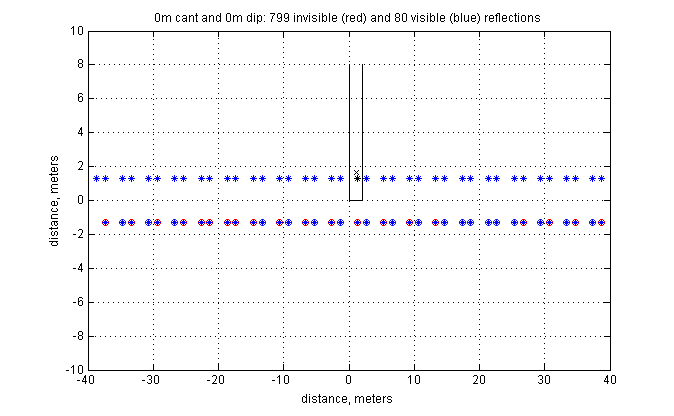
\includegraphics[width=\linewidth, trim=13mm 2mm 10mm 3mm, clip]{images/ISM_0m_cant_0m_dip.png} \caption{Virtual source locations for an alleyway with no canting. Note that invisible sources appear in the same locations as visible ones: for example, $vs_{02}$ and $vs_{20}$ are in the same location, but because the microphone is above the source, it ``sees" $vs_{20}$ and not the other. This illustrates the degeneracy of sources in the image method.} \end{figure}

\begin{figure}[h!] \centering 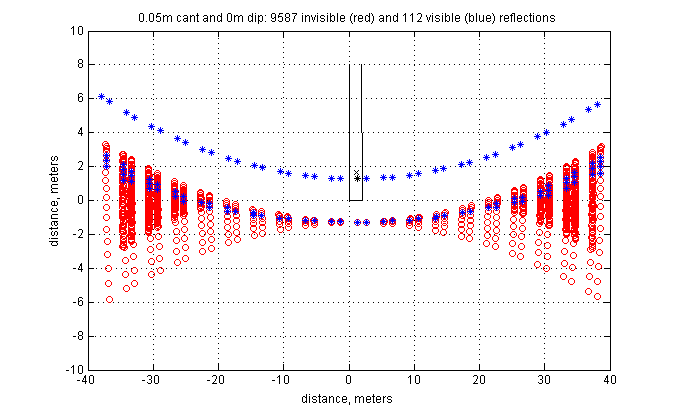
\includegraphics[width=\linewidth, trim=13mm 2mm 10mm 3mm, clip]{images/ISM_0pt05m_cant_0m_dip.png} \caption{Virtual source locations for an alleyway with both walls canted in 0.05m.} \end{figure}

\begin{figure}[h!] \centering 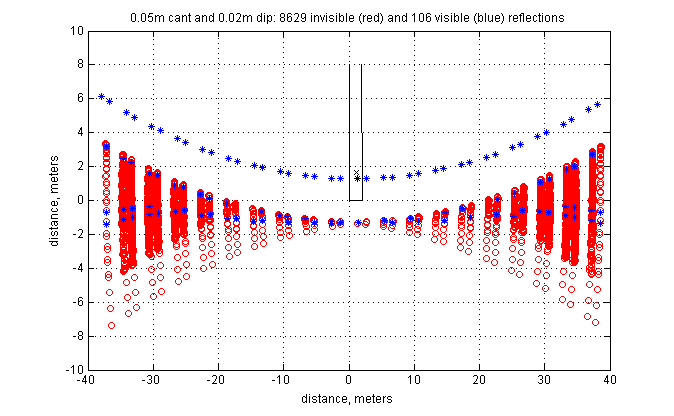
\includegraphics[width=\linewidth, trim=13mm 2mm 10mm 3mm, clip]{images/ISM_0pt05m_cant_0pt02m_dip.png} \caption{Virtual source locations for an alleyway with both walls canted in 0.05m and a dip in the center of the ground of 0.02m.} \end{figure}

These more complex constraints lead to a model with sources lying on a
circle centered where the two walls would meet in space were they
extended sufficiently long, then another circle of sources reflected
about the floor, and finally, dense arcs of sources that intersect
both of these circles at 90 degree angles.

\begin{figure}[h!] \centering 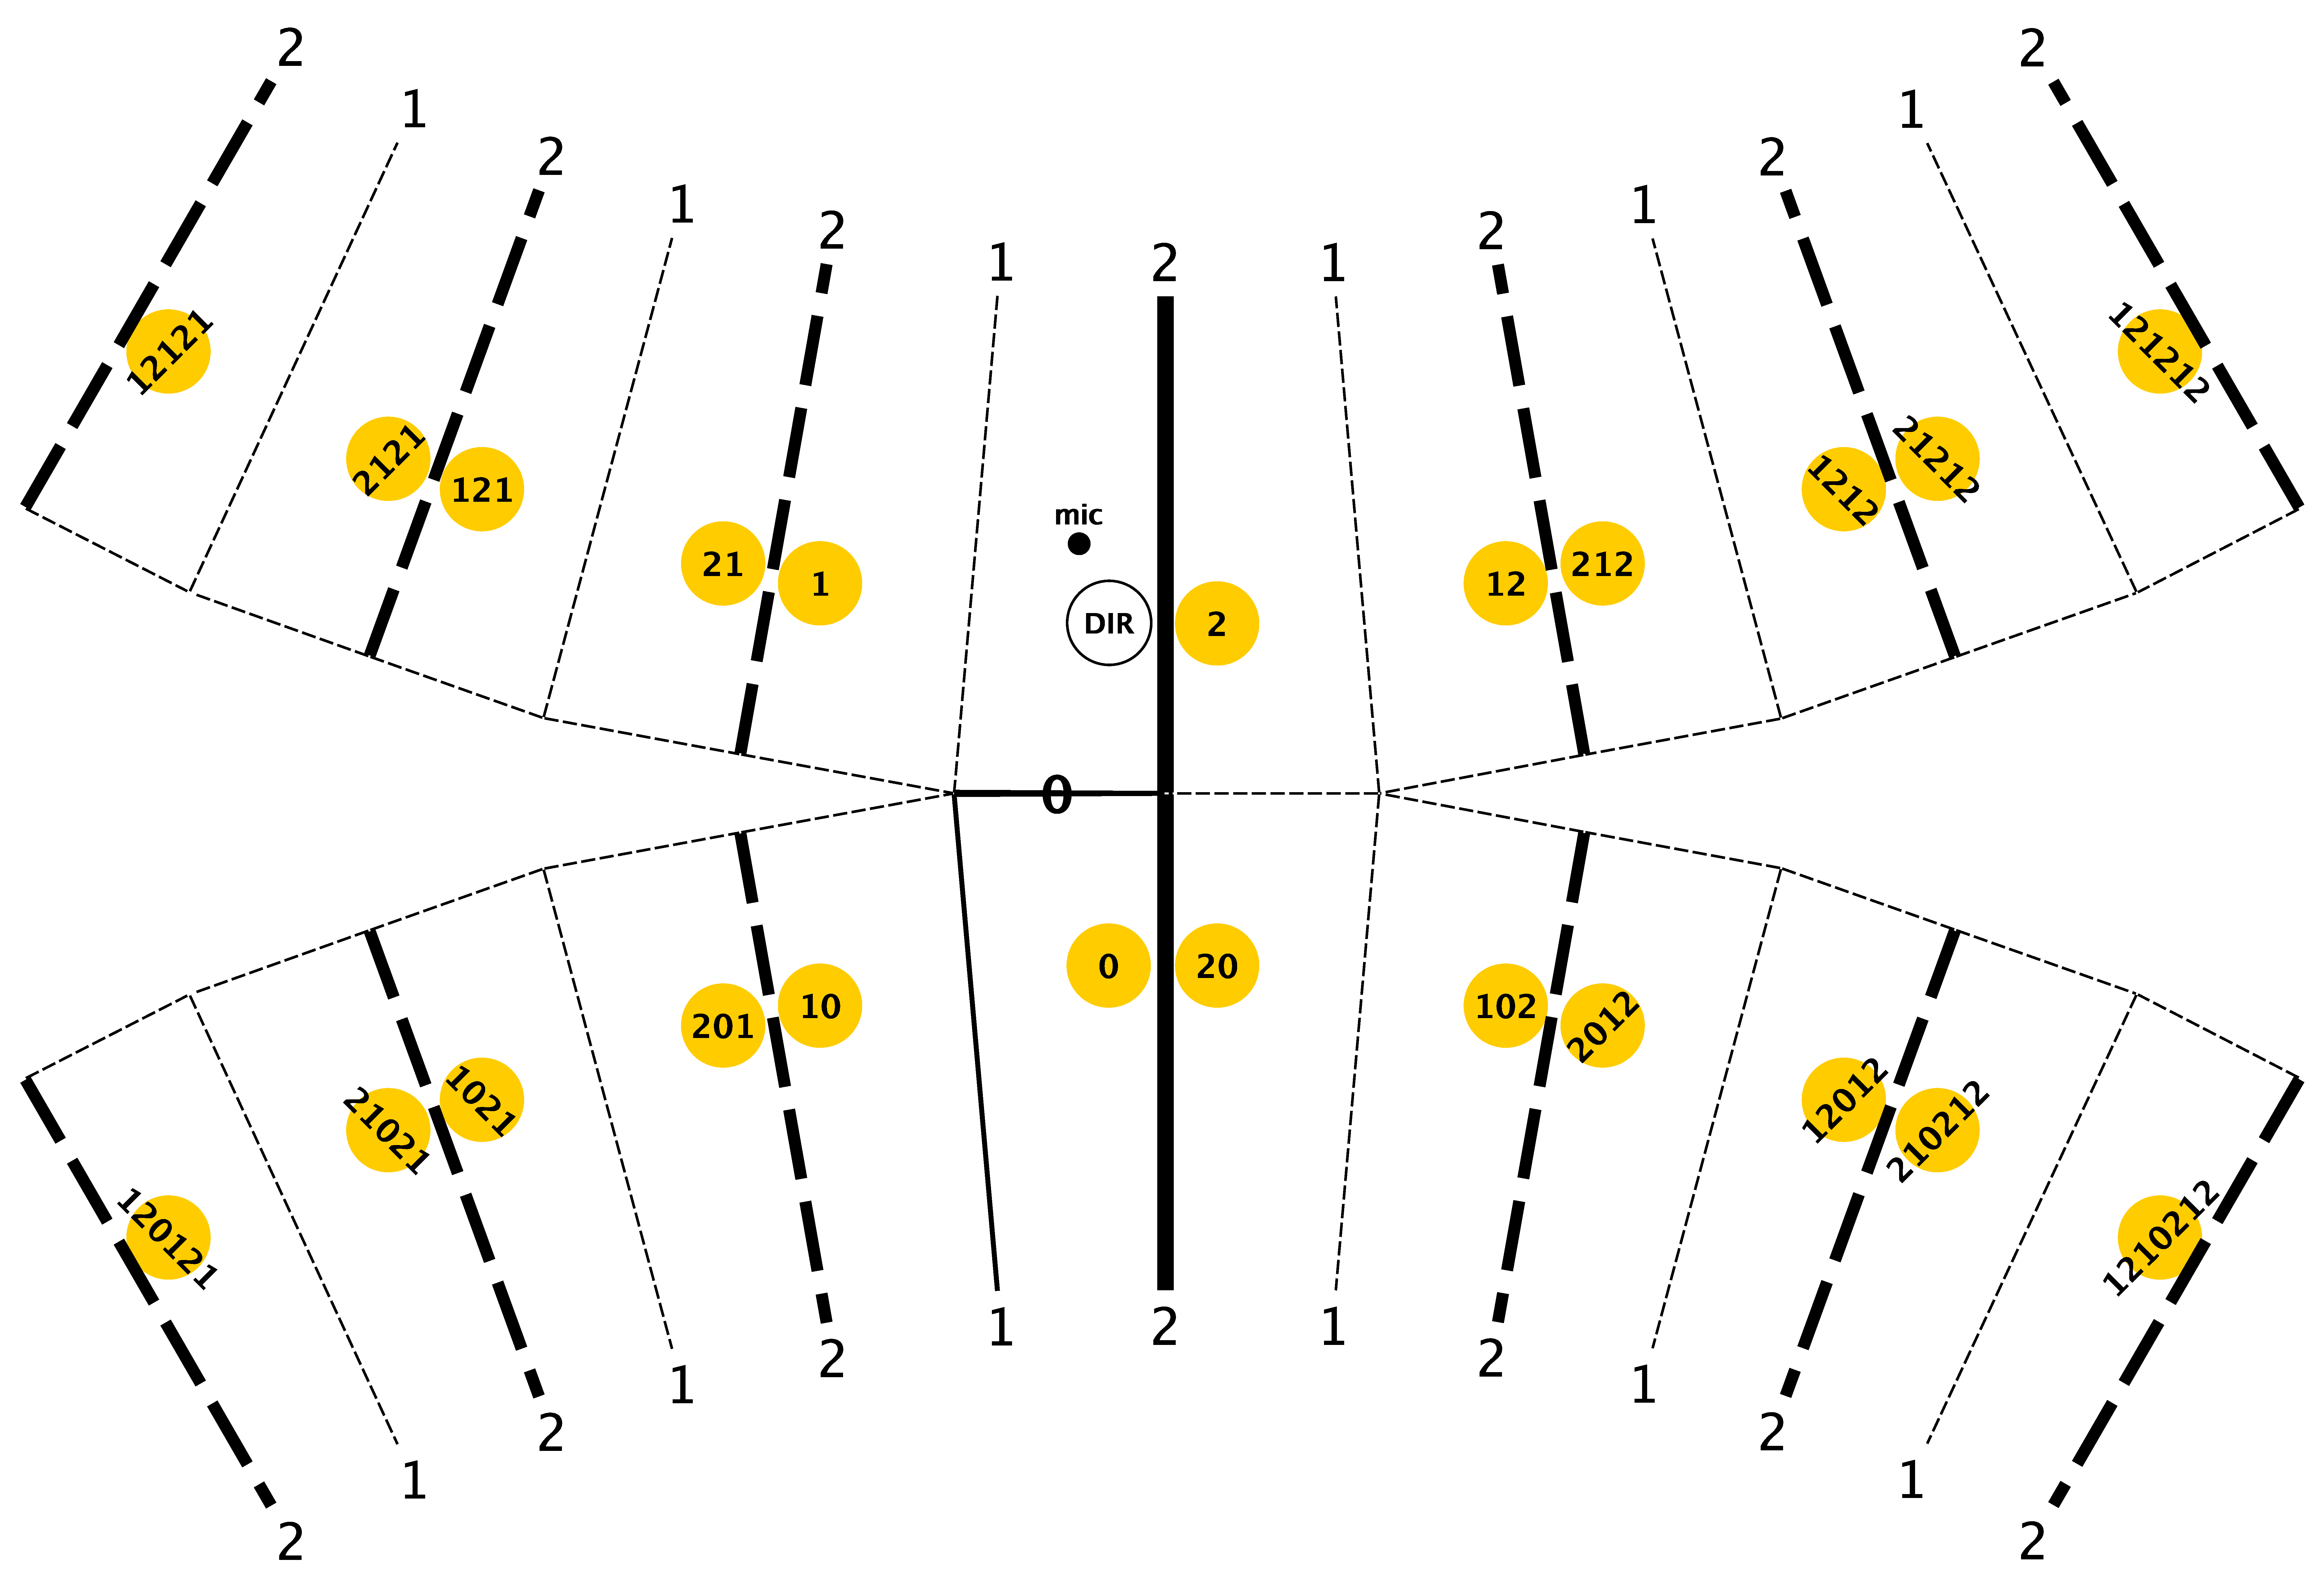
\includegraphics[width=\linewidth]{images/ISM_canted_v2.pdf} \caption{The image sources lie on a circle centered at the point of the wall intersection, if they were extended infinitely through space.} \end{figure}

These ``ripples" of concentric arcs generate the amplitude modulation
that we experience. The degree to which energy is reflected back into
the alleyway at its upper boundary is frequency dependent, and this
makes for frequency dependent modulation of a given mode.

Reflection filters for the walls consisting of painted concrete block
are virtually flat, but were accounted for according to the following
table.

\begin{table}
\begin{center} \small
\begin{tabular}{|l|c|c|c|c|c|c|}
\hline
$f$ (Hz) & 125 & 250 & 500 & 1000 & 2000 & 4000 \\
\hline
Gain & 0.9 & 0.95 & 0.94 & 0.93 & 0.91 & 0.92 \\
\hline
\end{tabular}
\caption{Absorption coefficients for painted concrete.} 
\end{center} \normalsize
\end{table}

\subsection{Synthesis}


\section{Evaluation and Conclusion}

Impulse responses generated from the image sources reproduce many of
the features of the measured alleyway responses. The harmonic series
and the spectral zeros rising in frequency over time are clearly
visible, and appear to be due to the changing listener arrival times
of signals from the image source row above the ground, relative to the
arrival times from the image source row below the ground.

The long lasting modulated tone is not present in the simple image
source model. While the open alleyway top would create an inverting
reflection, thus keeping energy in the alleyway, it would do so only
at frequencies much lower than that of the frequency of the long
lasting tone, which in our measurements is twice that of the inverse
wall spacing. If the alleyway walls are slightly canted inward, the
long lasting tone and its modulation can be produced. In this case,
the modulation can be thought of as a result of the time taken for
sound waves to reflect many times off the alleyway walls, be directed
downwards by the wall cant, and then reflect back upwards from the
ground.

\section{Acknowledgements}
Thanks to Sahar Tai-Seale and Dave Kerr.

%\begin{table*}
%\begin{center}
%\begin{tabular}{|c|l|r|}
%\hline
%234093241&23402312&3432829807434\\
%2398234&423403290&123144298\\
%2340243012597398&1245987533&24982499\\
%\hline
%\end{tabular}
%\caption{This is a two-column table.}
%\end{center}
%\end{table*}
%
%
%\begin{figure*}[tb!]
%\begin{center}
%\fbox{\vrule width0pt height 1in\vrule width6in height 0in}
%\end{center}
%\caption[2]{It is best to place to place two-column figures at the bottom
%or top of a page.}
%\end{figure*}

\begin{thebibliography}{99}

\bibitem{Borish}
Borish, J. ``Extension of the image model to arbitrary polyhedra." J. Acoust. Soc. Am. 75, 1827 (1984).
\bibitem{Morse}
Morse, P. and K. Ingard. \emph{Theoretical Acoustics}. Princeton, NJ: Princeton University Press, 1987, pp.~471, 503, 571.

%\bibitem{DEK2}
%D. E. Knuth, {\it Selected papers on analysis of algorithms}, CSLI
%Publ., Stanford, CA, 2000; CNO
%CMP 1 762 319 
%
%\bibitem{DEK3}
%D. E. Knuth, Algorithmica {\bf 22} (1998), no.~4, 561--568; MR
%2000j:68037 
%
%\bibitem{DEK4}
%R. L. Graham, D. E. Knuth and O. Patashnik, {\it Concrete mathematics}
%(Polish), Translated from the
%second English (1994) edition by P. Chrzastowski, A. Czumaj,
%L. Gasieniec and M. Raczunas, Second
%edition, Wydawnictwo Naukowe PWN, Warsaw, 1998; MR 99m:68002
%
\end{thebibliography}


\end{document}
